
\exercise{Going by bus}{4}
Suppose we want to go from A to D in the network shown below. Too boring? Well, this time we are going to take the bus, and now the weights specify the frequency of the bus connection between two places. So weight 1 means that the bus goes every hour. While for example the 4 between A and D means that the bus only goes every fourth hour. For simplicity all busses leave on the hour starting at 12:00 and each ride take slightly less than 3 hours. So if we take a bus at 2:00 we could catch a connecting bus at 5:00 (if one is leaving then). Find the optimal path from A to D, starting at 12:00, and then formulate a Dijkstra-style procedure that can solve this problem on general networks. Convince yourself that your proposed procedure will always find the optimal solution. 

\begin{center}
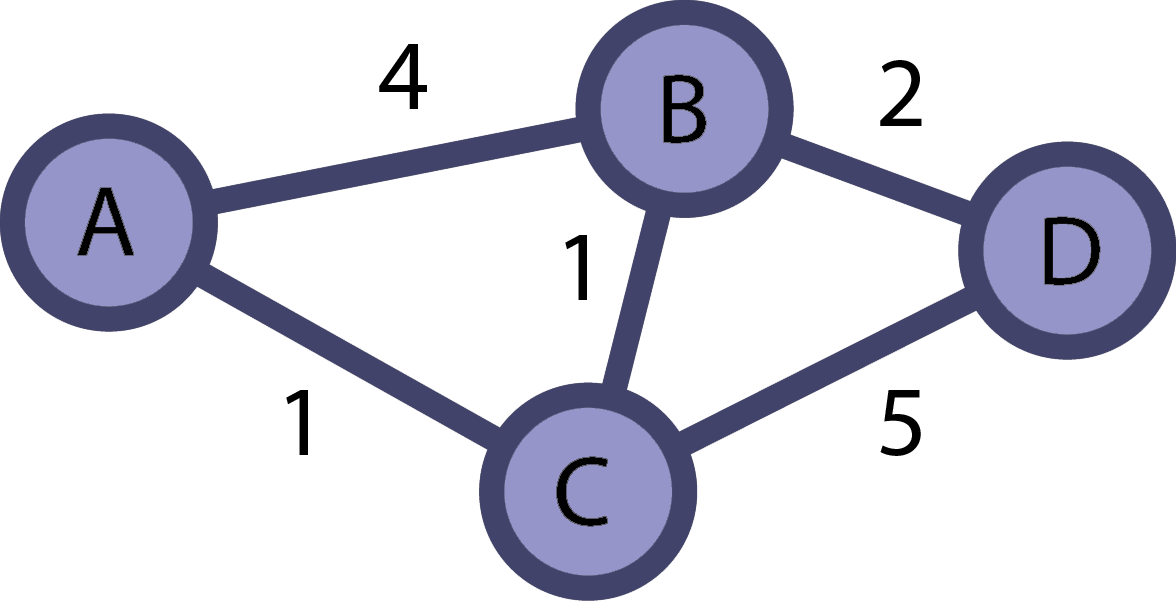
\includegraphics[width=0.3\textwidth]{hobbitmedium.png}
\end{center}

\solution 
The challenge here seems very similar to a typical Dijkstra question, so we solve it by basically applying Dijkstra's algorithm. However, since there are now some complications we will carefully go step by step and adapt the algorithm as necessary. We start by creating a table to record the upper bounds for the time by which we can be in a given place.   

\begin{center}
\begin{tabular}{c c c c}
A & B & C & D \\\hline 
12:00 & \oo & \oo & \oo \end{tabular}
\end{center}

Since we start at noon we can be sure that we can be at A by noon. For all other places our upper bound is infinity. Since we know the definite time by which we can be at A let's update from there: The bus to B only goes every 4 hours but fortunately there is one leaving right at 12:00, we could take it and be at B by 15:00 (or 3pm). There is also a bus leaving at 12:00 that would take us to C by 15:00. So our updated table is now 
\begin{center}
\begin{tabular}{c c c c}
A & B & C & D \\\hline 
12:00 & \oo & \oo & \oo \\
      & 15:00 & 15:00 & \oo \end{tabular}
\end{center}
We can now update from either B or C. I will stick to my convention and first update from the leftmost place in the list, so let's update from B. From B the bus to D leaves ever two hours. So the next one is leaving at 16:00 and arrives at D by 19.00. There is 
also a bus to C that goes every hour. If we took this bus from B to C we would arrive at C by 18:00, but we have already found a faster way to go to C, so we reject this update. Our table now reads  
\begin{center}
\begin{tabular}{c c c c}
A & B & C & D \\\hline 
12:00 & \oo & \oo & \oo \\
      & 15:00 & 15:00 & \oo \\
      &  & 15:00 & 19:00 \end{tabular}
\end{center}
So we have found a way to D but we can't be quite sure that it is the fastest one. To be sure let's update from C. We can be at C by 15:00, but the bus from C to D only leaves every 5 hours, so the next one is at 17:00. In this way we would get to D by 20:00, which is an hour slower that the way we have found already. So after this update we have \begin{center}
\begin{tabular}{c c c c}
A & B & C & D \\\hline 
12:00 & \oo & \oo & \oo \\
      & 15:00 & 15:00 & \oo \\
      &  & 15:00 & 19:00 \\ 
      &  &       & 19:00 \\       
      \end{tabular}
\end{center}
We can now be sure that the fastest way to D is the route A-B-D which takes us to the destination by 19:00 (7 pm). 

Although the rules were a bit more complicated in this case, the problem is still solvable by a procedure that is essentially Dijkstra's algorithm. Following the logic from the chapter we can convince ourselves that we can still find the optimal solution. 
